% !TEX root = ../paper.tex

This section presents results for a number of test problems, which compare
solutions obtained using:
\begin{itemize}
  \item the standard Galerkin FEM, titled in plots as ``Galerkin'',
  \item the low-order method, titled in plots as ``Low'',
  \item the entropy viscosity method, titled in plots as ``EV'',
  \item the standard Galerkin FEM with FCT, titled in plots as ``Galerkin-FCT'', and
  \item the entropy viscosity method with FCT, titled in plots as ``EV-FCT''.
\end{itemize}
All problems assume a speed of $v=1$ (the speed effectively just changes the
units of $\dt$), an entropy function of $\eta(u)=\frac{1}{2}u^2$, and entropy
viscosity tuning parameters of $c_\mathcal{R}$ and $c_\mathcal{J}$ are set
to 0.1. Unless otherwise stated, the transport direction is in the postive
$x$ direction: $\mathbf{\Omega}=\mathbf{e}_x$.

%===============================================================================
\subsection{Spatial Convergence}
%===============================================================================
This 1-D, steady-state test problem uses the Method of Manufactured Solutions (MMS) with
a solution of $u(x)=\sin(\pi x)$ on the domain $x\in(0,1)$. Zero Dirichlet
boundary conditions are imposed on both boundaries.
With $\sigma(x)=1$,
the MMS source becomes $q(x)=\pi\cos(\pi x) + \sin(\pi x)$.
The number of cells in the study began as 8 in the coarsest mesh, and cells
were refined by a factor of 2 in each cycle, ending with 256 cells.

Figure \ref{fig:mms_sinx_ss} shows the $L^2$ norm errors for this convergence study
and indicates first-order spatial convergence for the low-order method and
second-order spatial convergence for the entropy viscosity (EV) method
and EV FCT method, as expected.

\begin{figure}[htb]
   \centering
      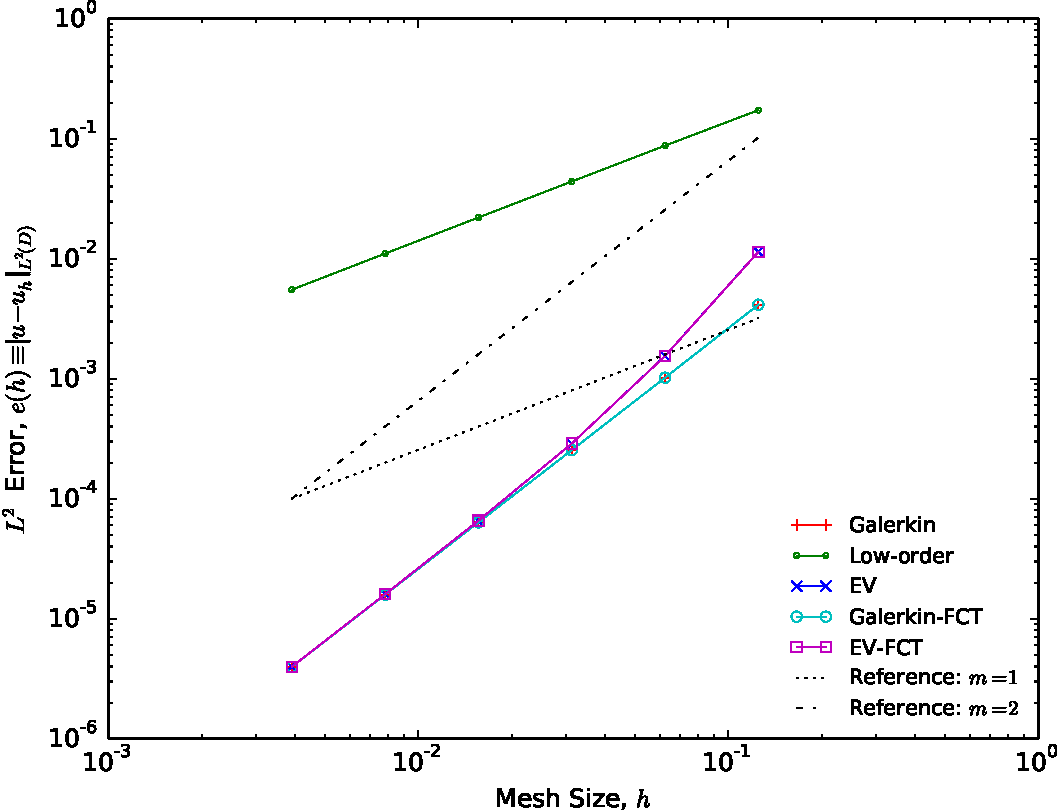
\includegraphics[width=\textwidth]
        {images/convergence_sinx.pdf}
      \caption{Spatial Convergence for MMS Problem}
   \label{fig:mms_sinx_ss}
\end{figure}
\clearpage
%===============================================================================
\subsection{Glancing Beam in a Void}
%===============================================================================
This 2-D test problem is on the unit square: $\x\in(0,1)^2$ and simulates
a beam incident on the bottom boundary of a void region
($\sigma(\x)= 0$, $q(\x)=0$) at a shallow angle of
$21.94^\circ$ with respect to the x-axis.
The exact solution of this problem contains a discontinuity along the line
$y = \frac{\Omega_y}{\Omega_x}x$, which presents opportunity for the formation
of spurious oscillations.
This was run as a transient problem with zero initial conditions but was run to
steady-state. A Dirichlet
boundary condition with a value of 1 is imposed on the bottom boundary
and a value of 0 on the left boundary.

This problem was run with Explicit Euler time discretization and a CFL
number of 0.5 on a $64\times64$ mesh. Figure \ref{fig:glance_in_void_fe}
compares the numerical solutions for this problem obtained with the
low-order, EV, Galerkin-FCT, and EV-FCT schemes. The Galerkin scheme
(without FCT) produced spurious oscillations without bound, so those
results are omitted here. The EV solution is much less diffusive along
the discontinuity, but contains spurious oscillations. Both FCT solutions
keep the solution within some physical bounds, but one can see from
the Galerkin-FCT results that some ``terracing'' effects are present; this
behavior is a well-known artifact of traditional FCT schemes \cite{kuzmin_FCT}.
The EV-FCT scheme, however, shows a significant reduction in this effect,
as expected; the addition of the entropy-based artificial viscosity
lessens the burden on the limiter. This result was found to be typical
when comparing Galerkin-FCT and EV-FCT, although there are some cases
when the difference is minimal, or even the Galerkin-FCT solution is slightly
superior due to less artificial diffusion.

\begin{figure}[ht]
   \centering
   \begin{subfigure}{0.45\textwidth}
      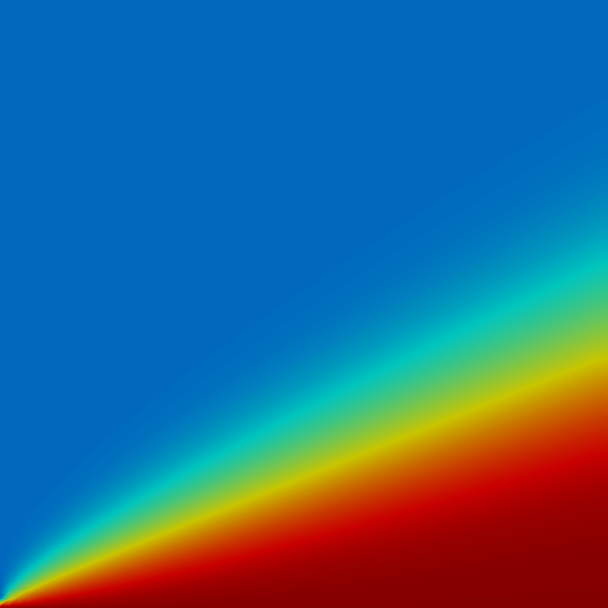
\includegraphics[width=\textwidth]
        {images/glance_Low.png}
      \caption{Low-Order}
   \end{subfigure}
   \begin{subfigure}{0.45\textwidth}
      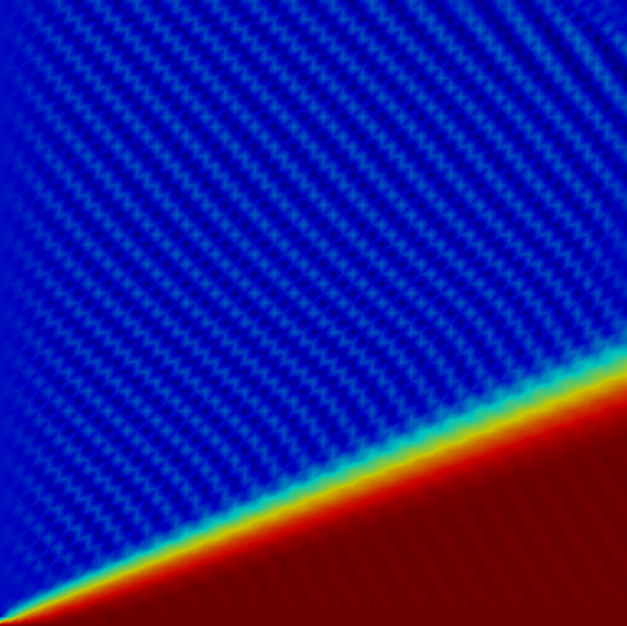
\includegraphics[width=\textwidth]
        {images/glance_EV.png}
      \caption{EV}
   \end{subfigure}
   \begin{subfigure}{0.45\textwidth}
      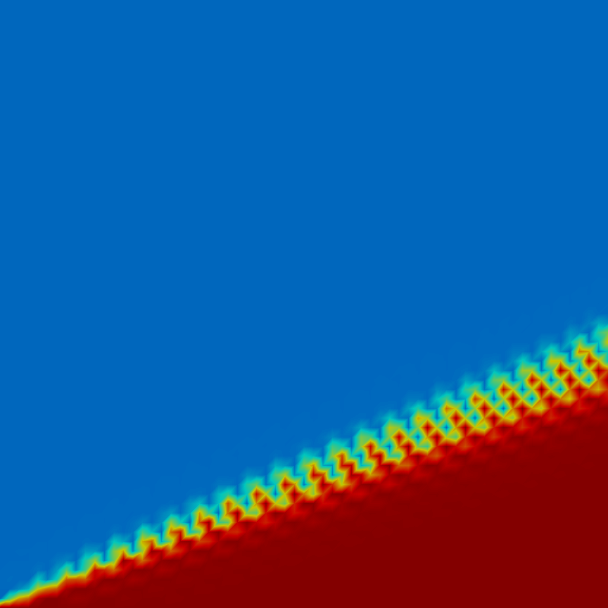
\includegraphics[width=\textwidth]
        {images/glance_GalFCT.png}
      \caption{Galerkin-FCT}
   \end{subfigure}
   \begin{subfigure}{0.45\textwidth}
      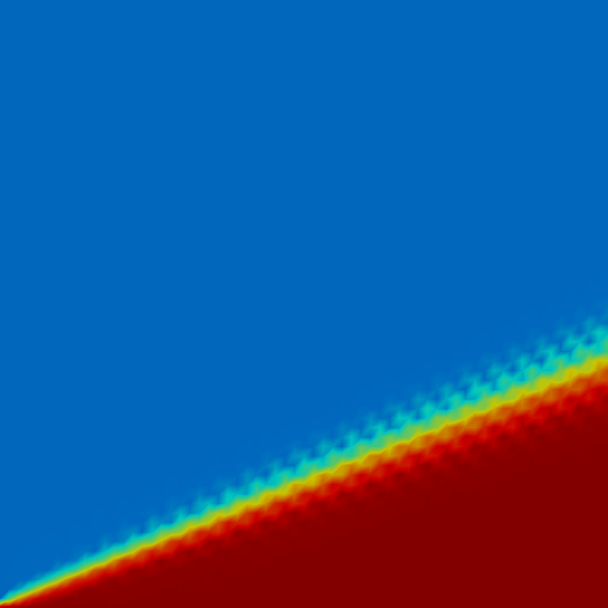
\includegraphics[width=\textwidth]
        {images/glance_EVFCT.png}
      \caption{EV-FCT}
   \end{subfigure}
   \caption{Comparison of Solutions for the Glance-in-Void Test
     Problem Using Explicit Euler Time Discretization}
   \label{fig:glance_in_void_fe}
\end{figure}
\clearpage
%===============================================================================
\subsection{Obstruction}
%===============================================================================
This is a 2-D, two-region problem on the unit square $(0,1)^2$ with a beam incident on the
left and bottom boundaries at an angle of $45^\circ$ with the x-axis. The
center region $(\frac{1}{3},\frac{2}{3})^2$ is an absorber region
with $\sigma(\x)=10$ and $q(\x)=0$, and the surrounding region is a void
($\sigma(\x)=0$, $q(\x)=0$).

This problem was run with Implicit Euler with a CFL of 1 to steady-state on
a $32\times32$ mesh. The results are shown in Figure \ref{fig:obstruction_be}.
The low-order solution is especially diffusive and shows a fanning
of the solution after it passes the corners of the obstruction, which is
not present in any of the high-order schemes. The EV solution contains
oscillations, although they are much less significant than in the Galerkin
solution. Both FCT schemes show a lack of these oscillations, but the
Galerkin-FCT solutions shows a terracing effect. The EV-FCT solution also
has this effect but to a much smaller degree.

\begin{figure}[ht]
   \centering
   \begin{subfigure}{0.3\textwidth}
      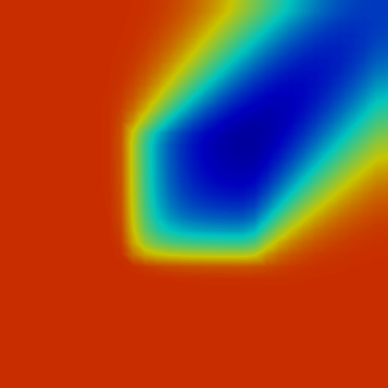
\includegraphics[width=\textwidth]
        {images/obstruction_low.png}
      \caption{Low-Order}
   \end{subfigure}
   \begin{subfigure}{0.3\textwidth}
      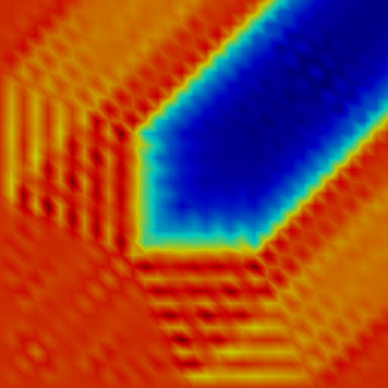
\includegraphics[width=\textwidth]
        {images/obstruction_Gal.png}
      \caption{Galerkin}
   \end{subfigure}
   \begin{subfigure}{0.3\textwidth}
      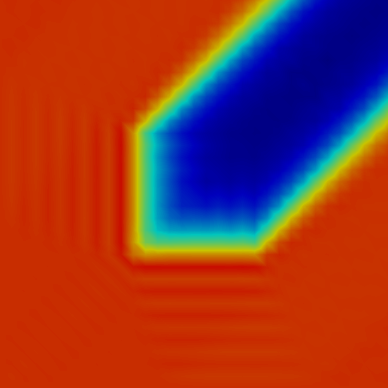
\includegraphics[width=\textwidth]
        {images/obstruction_EV.png}
      \caption{EV}
   \end{subfigure}
   \begin{subfigure}{0.3\textwidth}
      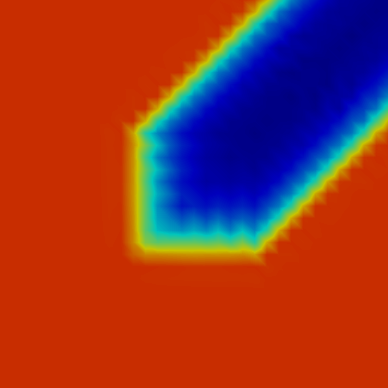
\includegraphics[width=\textwidth]
        {images/obstruction_GalFCT.png}
      \caption{Galerkin-FCT}
   \end{subfigure}
   \begin{subfigure}{0.3\textwidth}
      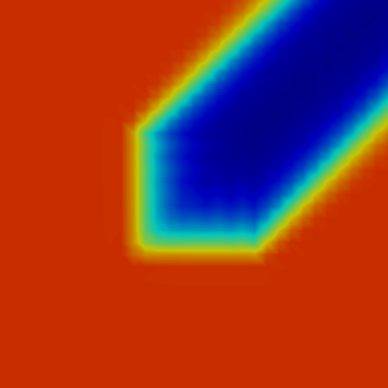
\includegraphics[width=\textwidth]
        {images/obstruction_EVFCT.png}
      \caption{EV-FCT}
   \end{subfigure}
   \caption{Comparison of Solutions for the Obstruction Test
     Problem Using Implicit Euler Time Discretization}
   \label{fig:obstruction_be}
\end{figure}
\clearpage
%===============================================================================
\subsection{Two-Region Interface}
%===============================================================================
This 1-D test problem simulates the interface between two regions with
varying cross section and source values on the domain $(0,1)$.
The left half has values $\sigma(\x)=10$ and $q(\x)=10$, giving it a
saturation value of $\frac{q}{\sigma}=1$, while the right half has values
of $\sigma(\x)=40$ and $q(\x)=20$, giving it a saturation value of
$\frac{q}{\sigma}=0.5$.

This problem was run using SSPRK33 time discretization with a CFL of 1 to
steady-state with 32 cells. Figure \ref{fig:interface} shows the results
for this test problem. The low-order solution suffers from the significant
artificial diffusion, while the Galerkin solution suffers from significant
spurious oscillation. The EV scheme eliminates some of the first oscillations,
but a number of oscillations of a similar magnitude to those produced by
the Galerkin scheme still exist to the left of the interface. Both FCT
schemes effectively eliminate spurious oscillations without approaching
the level of unnecessary artificial diffusion achieved by the low-order
scheme. For this test problem, the Galerkin-FCT solution is slightly
superior to the EV-FCT solution since the classic ``terracing'' phenomenon
of FCT is not present.

\begin{figure}[htb]
   \centering
      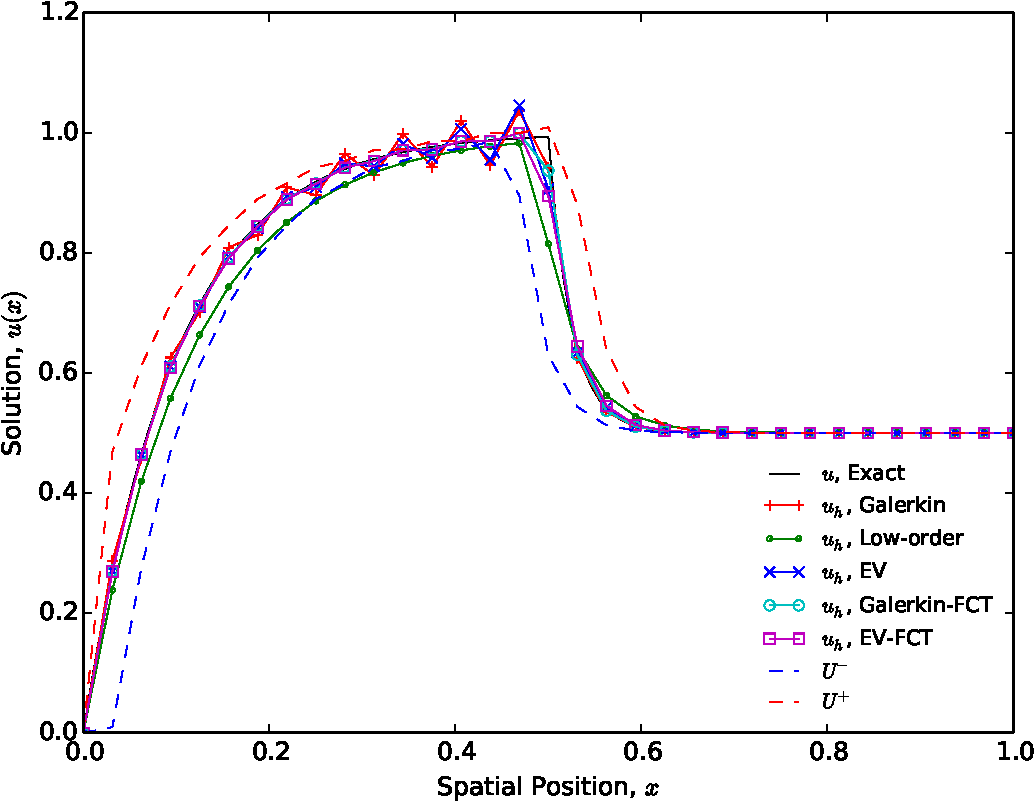
\includegraphics[width=\textwidth]
        {images/solution_interface.pdf}
      \caption{Comparison of Solutions for the Two-Region Interface Test
       Problem Using SSPRK33 Time Discretization}
   \label{fig:interface}
\end{figure}
\clearpage
%===============================================================================
\subsection{Source in a Void}
%===============================================================================
This 1-D test problem has two regions, the left being a void but with a source:
$\sigma(\x)=0$ and $q(\x)=1$, and the right being an absorber without a source:
$\sigma(\x)=10$ and $q(\x)=0$. This represents a non-physical problem since
a source is produced in a void, but nevertheless it represents a useful test
problem. A zero Dirichlet boundary condition is imposed on the incoming (left)
boundary, and this problem is run as a steady-state problem on the domain
$(0,1)$ with 32 cells.

Figure \ref{fig:source_in_void} shows the results for this problem.

\begin{figure}[htb]
   \centering
      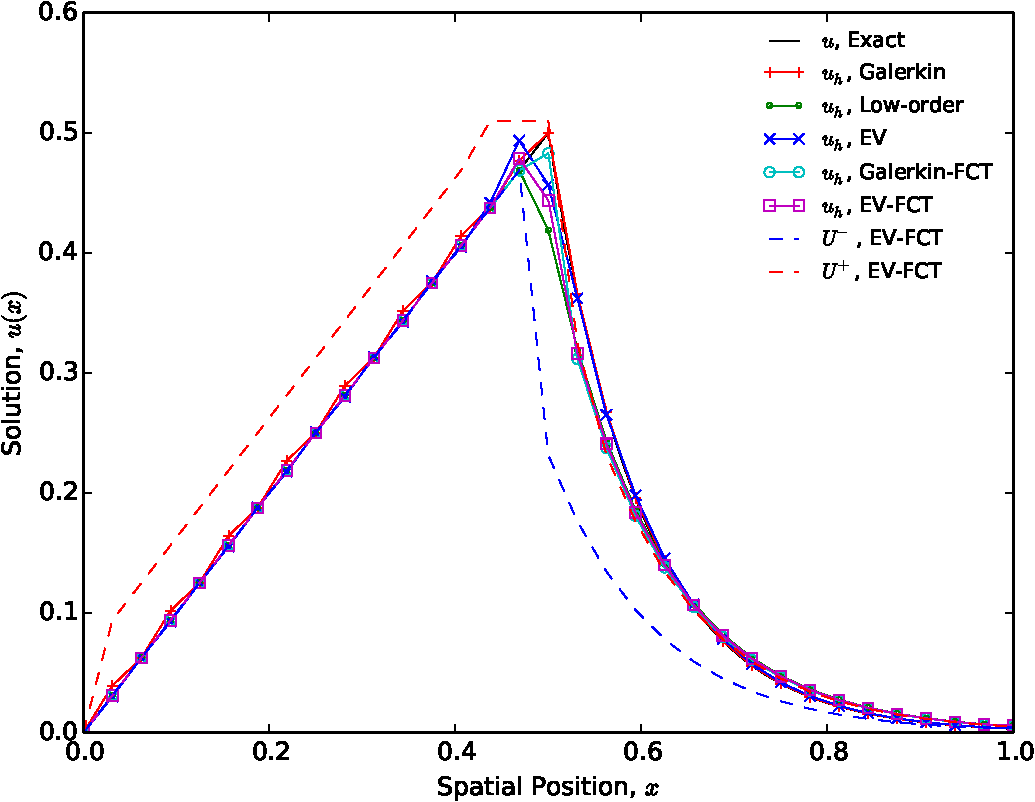
\includegraphics[width=\textwidth]
        {images/solution_source_in_void.pdf}
      \caption{Comparison of Solutions for the Source-in-Void Test
       Problem Using Steady-State Time Discretization}
   \label{fig:source_in_void}
\end{figure}
\clearpage
